
\section{工程概况}
\subsection{施工组织设计编制基本原则}

施工组织设计按照编制对象,可分为施工组织总设计、单位工程施工组织设计。
施工组织设计应包括编制依据、工程概况、施工部署、施工准备与资料配置计划、
施工进度计划、主要施工方法、施工管理措施、施工现场平面布置等主要内容;
施工组织设计的编制必须遵循工程建设程序,并符合下列原则:

\begin{itemize}

    \item [1)] 符合国家有关法律法规、现行规范,符合地方规程、行业标准的要求;

    \item [2)] 满足建筑施工合同或招标文件中关于建筑工程进度、质量、环境保护、职业健康、安全、工程造价等工程管理目标的要求;

    \item [3)] 积极开发、推广运用新技术、新工艺、新材料、新设备;

    \item [4)] 坚持科学的施工程序和合理的施工顺序,做到资源的优化组织和合理配置,采用流水施工和网络计划的方法,实现均衡施工,努力实现科学、合理的经济技术指标;

    \item [5)] 积极响应国家关于低碳、节能、环保方面的方针、政策;采取先进的技术和管理措施,推广建筑节能和绿色施工。

    \item [6)] 与建筑施工单位质量、环境、职业健康安全、项目管理规范四合一标准的有效结合,贯彻质量、环境、职业健康安全管理国家管理规范的要求;

\end{itemize}

\subsection{施工组织设计编制程序}

施工组织设计的编制程序应遵守如下流程:

(1)收集和熟悉编制施工组织总设计所需的有关资料和图纸,进行项目特点的施工条件的调查研究;

(2)计算主要工种工程的工程量;

(3)确定施工的总体部署;

(4)拟定施工方案;

(5)编制施工总进度计划;

(6)编制资源需求量计划;

(7)编制施工准备工作计划;

(8)施工总平面图设计;

(9)计算主要技术经济指标。应该指出以上顺序中有些顺序必须固定,不可逆转,如:

\quan{1} 拟定施工方案后才可编制施工总进度计划(因为进度的安排取决于施工的方案);

\quan{2} 编制施工总进度计划后才可编制资源需求量计划(因为资源需求量计划要反映各种资源在时间上的需求)

施工组织设计的编制程序流程图见图 \ref{fig:c1f1}

\begin{figure}[thbp!]
    \centering
    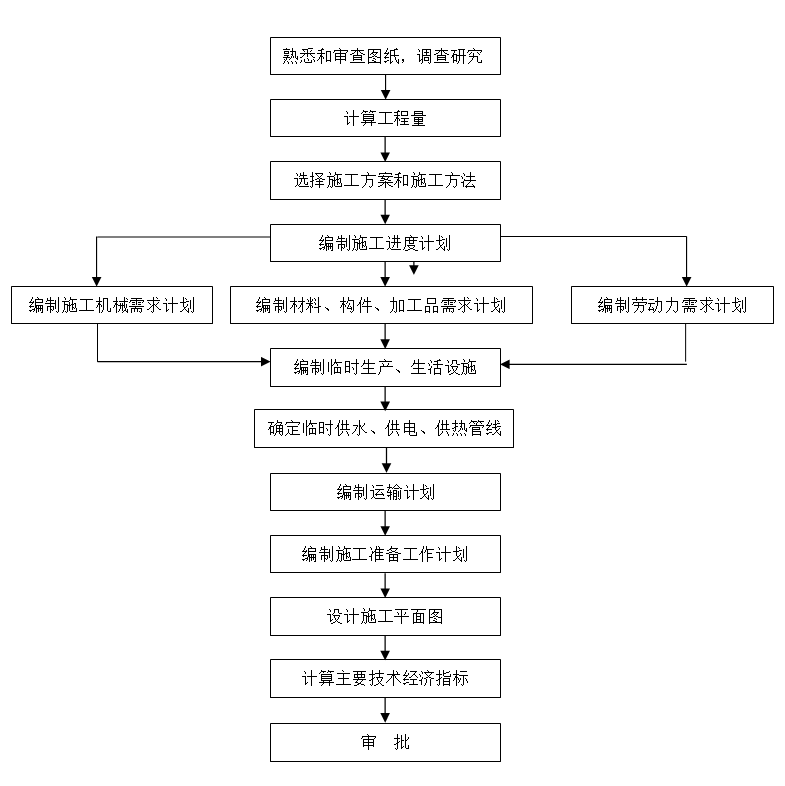
\includegraphics[width=1.0\linewidth]{figure/c1f1.png}
    \caption{单位工程施工组织设计编制程序}
    \label{fig:c1f1}
\end{figure}

\subsection{指导方针及编制依据}

\subsubsection{指导方针}

(1) 主要指导方针\\

为保证在计划工期内圆满地完成施工任务,本施工组织设计的主要指导方针是“服务至上,质量争先,科技先导,管理一流”。\\

(2) 科学组织、精心施工\\

组建一个高效团结的工程项目部和一支技术熟练、作风过硬的施工队伍,运用先进科学的现代化管理手段,
调动企业人力、物力、机械设备等各方面的优势资源,精心组织,与甲方、监理、各专业施工单位、工种密切配合,
根据工期进度要求,从图纸设计、现场测量、材料组织、现场施工、质量检验实行流水节拍式循环作业,
确保工程顺利按时完工。\\

(3) 质量第一、安全至上\\

制定严格的质量保证制度,充分考虑国家现行有关施工质量验收规范、标准和规定的要求,
从人员、材料、机械、环境等方面采取保证质量的措施,实施全员质量管理,确保工程质量达到预定目标。
建立完善的安全保证体系,制定严格的安全管理制度,遵守有关施工安全、防火、环卫的法律、法规,
坚决杜绝重大伤亡事故的发生,保证安全施工、文明施工。\\

(4) 科技先导、争创一流\\

采用先进的施工技术,科学合理地确定施工方案,在确保施工质量和效果的前提下,提高材料利
用率和工作效率,降低施工成本,提高经济效益。

\subsubsection{编制依据}

施工组织设计应以下列内容为主要编制依据:

\begin{itemize}

    \item [1)] 与建筑工程有关的法律、法规和相关文件;

    \item [2)] 国家现行有关标准、规范和技术经济指标;

    \item [3)] 工程所在地的行政主管部门的管理要求;

    \item [4)] 建筑施工行业相关的的质量、环境、职业健康安全管理体系管理规范的要求;

    \item [5)] 工程施工合同及招投标文件;

    \item [6)] 工程设计文件;

    \item [7)] 项目周边环境、现场条件、工程地质和水文、气象等自然条件;

    \item [8)] 与工程项目施工有关的资源供应、生产要素配置情况;

    \item [9)] 施工单位的生产能力、机具设备状况、技术水平等等。
    
\end{itemize}

\subsection{工程概况}
\subsubsection{建筑设计概况}

本工程名称为河南省旅游服务中心,建设地点为河南省郑州市,用地面积为 33333 平方米,总建筑面积为 29175 平方米,其中地上建筑面积 21332 平方米,其中地上建筑面积
地下建筑面积为 7843 平方米,建筑占地面积 8116 平方米,建筑高度 36 米,地上五层,地下一层;本工程为一类高层
建筑,建筑耐火等级为一级,设计使用年限为 50 年。

\subsubsection{结构设计概况}

本工程建造于河南省郑州市郑东新区,拟建层数地上五层,地下一层,主体结构高度 32.25m。
本工程的结构性质为 A 级高度高层建筑,结构体系为钢筋硂框架——剪力墙结构,使用年限 50 年
安全等级二级,主体结构采用桩基,设计等级甲级,基础安全等级二级。结合本工程所处地理位置,建筑
抗震设防类别为丙类,抗震设防烈度为 7 度。

\subsection{气象地质特点}
\subsubsection{气象特点}

郑州市位于河南省中部地区, 属暖温带亚湿润季风气候。四季分明,雨热同期,干冷同季。随着四季更替,依次呈现春季干旱少雨,
夏季炎热多雨,秋季晴朗日照长,冬季寒冷少雨雪的基本气候特征。年平均气温 14.3° C,7 月最热,平均 27°C;1 月最冷,
平均 0.1°C;年平均降雨量 632 毫米,无霜期 220 天,全年日照时间约 2400 小时。适宜的温度条件,充足的光照和农作物生长季节较为丰沛的雨量,构成了良好的农业气象条件。

\subsubsection{地质特点}

郑州市,位于东经 112°42'-114°13' ,北纬 34°16'-34°58',山地面积约 2377 平方公里, 水面面积约 11.4 平方公里。郑州北临黄河,西依嵩山,东南为广阔的黄淮平原,
东面是七朝古都东京开封市,西面为十三朝古都洛阳市,南面是许昌市,北面为焦作市和新乡市。郑州市横跨中国二、三级地貌台阶,西南部嵩山属第二级地貌台阶前缘,
东部平原为第三级地貌台阶的组成部分,山地与平原之间是低山丘陵地带。郑州最高点位于登封市的少室山,连天峰海拔约 1512.4 米;最低点位于中牟县韩寺镇胡辛庄,
海拔73米。邙山位于郑州市西北隅,邙山的地貌主要为黄土台地和黄土丘陵,由于黄河的侧蚀和众多沟谷侵蚀作用,使得黄土丘陵形态显得异常陡峻。

郑州地区位于丘陵岗地与泛滥平原相交接地带,为华北的平原一部分。地形比较平坦,地势由西南向东北倾斜。郑州区内地貌类型复杂多样,按其形态区内地貌依次分为:
丘陵岗地,波状平原,倾斜平原及泛滥平原。